

\chapter{Shock capturing}

As we saw in Ch.~\ref{ch:shocks}, the nonlinear term in Burger's
equation leads to trouble. Even the most innocent, small amplitude
wave, if left to run to $t \rightarrow \infty$ according to the compressible
Euler equations, will end up producing an infinite velocity
gradient -- otherwise known as a shock. Conservation of
mass, energy and momentum across the jump (the Rankine-
Hugoniot conditions) reveals a wonderful quirk of physics —
that differential equations with apparently no dissipation can
result in irreversible conversion of kinetic energy into heat
(i.e., entropy production).

All numerical methods for solving the Euler equations must
therefore deal with the inevitable formation of discontinuities.
That is, they must provide a mechanism for irreversible
dissipation at shock fronts.

In this chapter we will deal with some of these methods. 

\section{Bulk viscosity}

Perhaps the simples way to deal with discontinuties was proposed by Von Neumann
\& Richtmyer (1950), add an ``artificial viscosity''
term that acts on the shortest resolvable length scale in the
calculation, performing the role that microscopic viscosity
plays in Nature. In their model the viscosity is artificial
because the coefficient depends on resolution, as an extra pressure.

High-order non-conservative methods usually use this prescription,
borrowing a concept from non-ideal gases, which is the notion
of {\it bulk viscosity}, also referred to as volume viscosity, or second
viscosity. It represents the fluid's resistance to
compression, which microphysically stems from the finite
time it takes for energy given to the fluid to be distributed to the
rovibrational molecular modes. Monoatomic gases and ideal gases do not have bulk
viscosity.

Another way to think of second viscosity is the dissipation that
happens while the gas is out of equilibrium following an expansion or
compression event. Usually the restoration of equilibrium is fast, but
if the relaxation time is long, dissipation will occur. 

Its general form in the NS equation is to add a term to the viscous
tensor that is proportional to the flow divergence

\beq
\pi_{ij}=[...] - \rho\zeta \delta_{ij} \Div{\v{u}}
\label{eq:pizeta}
\eeq

With corresponding acceleration 

 \beqn
 f_\nu(u,\rho) &=& -\rho^{-1}\Div{\v{\pi}} \\
 &=&\zeta\left[ \grad{\left(\Div{\v{u}}\right)} + \left(\grad{\ln\rho}+\grad{\ln\zeta}\right) \Div{\v{u}}\right]
\label{eq:zeta-acceleration}
 \eeqn

% But what does it have to do with discontinuities? As it turns out,
% volume viscosity behaves much as we expect dissipation in a shock to behave. In any
% rapid process, the fluid deviates from equilibrium, but quickly
% returns to it. If, however, the time to return to equilibrium is
% long, dissipation can happen during this long expansion or
% compression. 
  
%div(nu_shock*grad(uu_i))

% tmp=nu_shock*(p%shock*(p%divu*p%glnrho+p%graddivu)+p%divu*p%gshock)

Using a bulk viscosity to deal with shocks in numerical schemes was
first proposed by von Neumann \& Richtmyer (1950). The idea is to add
an artificial viscosity that acts on the shortest resolvable length
scale in the grid. This artificial bulk viscosity will simply smooth a
 discontinuity to a width that can be resolved by the stencil \figp{fig:shock-viscosity}. As long
 as the shock viscosity coefficient can be written in the form
 \eq{eq:pizeta} so its divergence is taken to find the acceleration
 \eq{eq:zeta-acceleration}, the term conserves momentum. 

\begin{figure}
  \begin{center}
    \resizebox{\textwidth}{!}{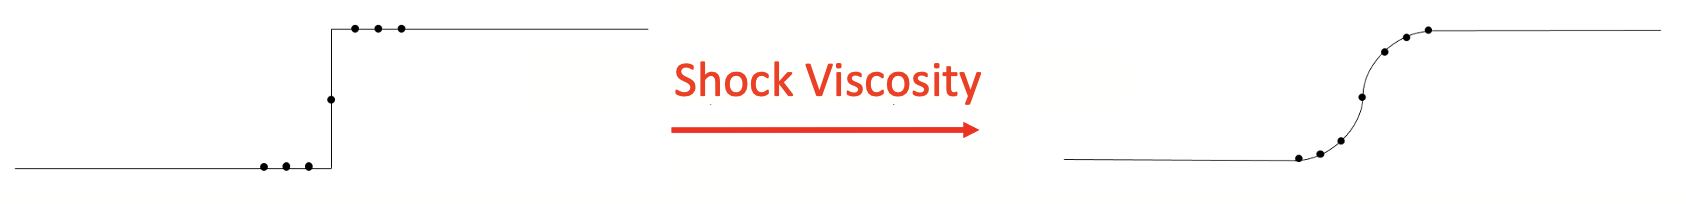
\includegraphics{./figs/shockviscosity.png}}
  \end{center}
  \caption[]{Shock viscosity is used to smooth a discontinuity to the
    point it can be resolved by the stencil.}
  \label{fig:shock-viscosity}
\end{figure}

Consider a constant bulk viscosity coefficient, so that

\beq
\frac{\partial \v{u}}{\partial t} = \zeta\grad{\left(\Div{\v{u}}\right)} 
\eeq

\noindent as is, this is not what we want, since this formulation
operates on both expansion and compression. We want the
force to be zero for expansion ($\Div{\v{u}} > 0$), and activate only for
compression ($\Div{\v{u}}<0$). Thus, the make the $\zeta$ coefficient
proportional to the convergence part only

\beq
\zeta \propto \left(-\Div{\v{u}}\right)_+ 
\eeq

where the $+$ subscript says that only the positive part is
considered. It work as $f(x) = {\rm max}(0, x)$. As such, the
coefficient is

\beq
\zeta \propto \left\{
  \begin{array}{ll}
       -\Div{\v{u}}& {\rm if} \quad -\Div{\v{u}} >0 \\
      0 & {\rm if} \quad -\Div{\v{u}} < 0 \\
\end{array} 
\right.
\eeq

We can define a coefficient of shock viscosity $\nu_{\rm sh}$ to replace the
proportionality. To keep this coefficient close to unity, we will
normalize it by $\Delta x^2$ (since the artificial viscosity operates
on the Laplacian) 


\beq
\boxed{
  \zeta = \nu_{\rm sh}\left(-\Div{\v{u}}\right)_+ \Delta x^2
  }
\eeq

This is the form of the artificial shock viscosity proposed by von
Neumann \& Richtmyer. The acceleration due to shock viscosity is therefore

 \beqn
 f_\nu(u,\rho) &=& -\rho^{-1}\Div{\v{\pi}} \\
 &=&\zeta\left[ \grad{\left(\Div{\v{u}}\right)} + \left(\grad{\ln\rho}+\grad{\ln\zeta}\right) \Div{\v{u}}\right]
 \eeqn

Such a viscosity scheme ensures that energy is dissipated in regions
of the flow where shocks occur, whereas more quiescent regions are
left untouched. Notice that the acceleration is quadratic on the
divergence, so it will be stronger in shock regions than on the smooth
flow. 

The formulation for shock diffusion is similar, yielding

\beq
 f_D(\rho) = \zeta\left(\Laplace{\rho} + \grad{\ln\zeta}\cdot\grad{\rho}\right)
\eeq

This artificial viscosity has the good property that it only becomes
strong when its presence is required, and becomes negligible when the
flow is smooth. It is therefore much better than an uncontrolled
numerical diffusivity. As such, the von Neumann-Richtmyer artificial
viscosity, and varieties thereof, is used in a great many numerical hydrodynamics codes.

A few problems with the scheme are: the viscosity
affects the pre-shock region and the shock is therefore not as sharp
anymore as we had before. Also, it is not sufficient to completely
eliminate post-shock oscillations. Only a linear term can achieve
that, which is Godunov's theorem: 

{\it Linear numerical schemes for solving partial differential equations that do not generate
new extrema (i.e., preserve monotonicity), can be at most first-order accurate.}

%reduces the order of the scheme,
%since at the discontinuity only first order is achieved. 


The high-order schemes presented so far are the ``road less
traveled''.  Some hydrodynamics codes are based on such higher-order
numerical derivatives, like the {\it Pencil Code} that I
develop. Colloquially it is usually said that higher-order
schemes are more accurate than lower-order schemes.
However, this is only true if the function $f(x)$ is reasonably
smooth over length scales of order $\Delta x$.
In other words: the ${\mathcal O}(\Delta x^4)$ is only significantly
smaller than ${\mathcal O}(\Delta x^2)$ if $\partial^5_xf(x)\Delta x^4
\ll \partial^3_xf(x)\Delta x^2 \ll \partial_x f(x)$. That is, if the
higher order derivatives are smaller compared to the lower order
ones: {\it if the function is smooth}.
Higher-order schemes are therefore useful for flows that have no strong
discontinuities in them. This is often true for subsonic flows,
i.e. flows for which the sound speed is much larger than the typical
flow speeds. For problems involving shock waves and other types of
discontinuities such higher-order schemes turn out to be worse than
lower order ones. 

\section{Godunov schemes}

The standard
approach to grid-based astrophysical hydrodynamics is to use the
conservation form of the equations of motion 

\beq
\frac{\partial q}{\partial t} + \Div{f(q)} = 0 
\label{eq:flux-godunov}
\eeq

where here we changed the notation: $q$ for quantity, and $f(q)$ for
flux of the quantity. We will also introduce the concept of {\it cells}. The idea of flux conserving schemes is to create cells out of the grid, instead of just sampling grid
points. The grid points now become cell centers located at $x_i$, and
we now have cell interfaces or cell walls located at the
half-points. In 3D the cells can  be regarded as control volumes
containing our conserved quantities. 

Let us consider the 1D version of \eq{eq:flux-godunov}

\beq
\frac{\partial q}{\partial t} + \frac{\partial f}{\partial x} = 0 
\label{eq:flux-godunov-1D}
\eeq

and integrate it in time and space

\beq
\int_{x_1}^{x_2}\int_{t_1}^{t_2}\frac{\partial q}{\partial t} +
\frac{\partial f}{\partial x} dx dt = 0 
\eeq

bracketing the time evolution of $q$ and space evolution of $f$

\beq
\int_{x_1}^{x_2}\left[\int_{t_1}^{t_2}\frac{\partial q}{\partial t}dt\right]dx +
\int_{t_1}^{t_2}\left[\int_{x_1}^{x_2}\frac{\partial f}{\partial x} dx \right]dt = 0 
\eeq

the bracketed are substituted by the quantities themselves

\beq
\int_{x_1}^{x_2} \left[q(t_2)-q(t_1)\right] dx +
\int_{t_1}^{t_2}\left[f(x_2)-f(x_1) \right]dt = 0 
\eeq


%Let us discretize \eq{eq:flux-godunov}. With an Euler time discretization it yields

%\beq
%\frac{q_i^{n+1}-q_i^{n}}{\Delta t} = -\frac{\left( f_{i+\sfrac{1}{2}}  - f_{i-\sfrac{1}{2}}    \right)}{\Delta x} 
%\eeq

%where
we define the value at point $i$ as the average value of the
quantity integrated over the cell 

\beq
q_i^n = \frac{1}{\Delta x} \int_{x_i-1/2}^{x_i+1/2} q(x,t^n) dx 
\eeq

So we identify $x_1 = x_{i-1/2}$ and $x_2 = x_{i+1/2}$ as cell interfaces.

Similarly, for the time integrals

\beq
f_i^{n+1/2} = \frac{1}{\Delta t} \int_{t^n}^{t^{n+1}} f(x_i,t) dt 
\eeq


%in this form, we can cast the equation as

%\beq
%\int_{x_i-1/2}^{x_i+1/2}\int_{t^n}^{t^{i+1}} \left[\frac{\partial \v{u}}{\partial t} + \frac{\partial\left[F(\v{u})\right]}{\partial x} \right] dx dt = 0  
%\eeq

%so we the fluxes should be computed at the midpoint in time 

we end up with the advection problem in flux-conserving form.

\beq
q_i^{n+1} = q_i^{n}-\frac{\Delta t}{\Delta x} \left[ f^{n+1/2}_{i+\sfrac{1}{2}}  - f^{n+1/2}_{i-\sfrac{1}{2}}    \right]
\label{eq:advect-conserve}
\eeq

%where we define the time-averaged flux function as

%\beq
%F^{n+1/2}_{i+\sfrac{1}{2}} = \frac{1}{\Delta t} \int_{t^n}^{t^{n+1}} F(x_{i+1/2},t) dt 
%\eeq


%\eq{eq:advect-conserve} is the 

%%%% Price's text

%The key insight is to compute the flux at the interface between two
%adjacent cells. The idea of Godunov methods is to compute this flux by
%considering adjoining cells as the left and right states of a
%Riemann problem. In Godunov’s original method, one considers every pair of
%cells to be a shock. This results in a first order scheme by
%virtue of Godunov’s theorem. The way around this 
%is to no longer consider the values $\v{u}$ in the left and right states
%as constant, but instead to use the gradients to reconstruct the
%values of $\v{u}$ at the interface. In smooth flow, the reconstruction
%is exact and no dissipation occurs — because there is no
%jump in the fluid variables to produce irreversible dissipation.
%Reconstruction thus restores higher order convergence of the
%scheme in smooth flow. However, by Godunov’s theorem it is
%impossible to provide second order accuracy at shocks without
%re-introducing post-shock oscillations. So reconstruction is
%done with ``slope-limited'' gradients to ensure that the scheme
%remains monotone (i.e., does not introduce new maxima or
%minima). Slope limiters thus revert to the required first order
%accuracy when the gradients are discontinuous.

%When reconstruction is employed, it is no longer necessary
%to exactly solve the Riemann problem. For many applications
% an approximate solution will suffice, even though approximate
% Riemann solvers are more dissipative than exact solvers.

%% 
 
Since we (by definition of the fact that we solve a numerical problem) do not know exactly what
this average state is, it is the task of the algorithm to provide a recipe that estimates this as well
as possible. In the two examples below we shall describe two such algorithms.
 
 %because, for example, the above assumes that every discontinuity
%is a shock, rather than considering shocks, rarefactions and
%contact discontinuities separately. 

%The simplest ``approximate Riemann solver'' uses the ``local Lax-Friedrichs'' flux
%given by

\subsection{Donor-cell advection}

The simplest flux conserving scheme is the donor-cell scheme. In this scheme the ``average
interface state'' is simply $\tilde{q}_{i+1/2} \approx q_i$, i.e. the value of the
upwind cell. 

\beq
f_{i+1/2}^{n+1/2} \approx q_i^n u_{i+1/2}
\eeq

The physical interpretation of this method is the following. One assumes that the density is
constant within each cell. We then let the material flow through the cell interfaces, from left to
right. Since the density to the left of the cell interface is constant, and since the
CFL condition makes sure that the flow is no further than 1 grid cell spacing at maximum, we
know that for the whole time between time $t_n$ and time $t_{n+1}$,
the flux through the cell interface $\tilde{q}_{i+1/2} ^n u_{i+1/2}
\approx q_i^n u_{i+1/2}$ is constant. Once the time step if finished, the state
in each cell has the form of a step function. To get back to the original sub-grid model
we need to average the quantity $q(x)$ out over each cell, to obtain the new $q^{n+1}_i$ . This is what
happens in the donor-cell algorithm.

Notice that the scheme is very similar to the upwind scheme, in fact
identical if the velocity is constant, yielding the recurrence
relation

\beq
q_i^{n+1} = (1-C)q_i^n  + Cq_{i-1}^n
\eeq

The Donor-Cell algorithm is easily implemented
but, as the upstream differencing method, it is very diffusive.

\subsection{Slopes of the donor cell: Piecewise linear methods}

The donor-cell algorithm is a simple algorithm based on the idea that at the beginning of each
time step the state within each cell is constant throughout the cell. The state at the grid
center is therefore identical to that in the entire cell. The idea that the state is constant in the cell
is, however, just an assumption. One must make some assumption, because evidently we have
not more information about the state in the cell than just the cell-center state. But one could
also make another assumption. One could, for instance, assume that the state within each cell
is a linear function of position. One says that the state is assumed to be piecewise linear. The assumption that it is a linear function within the cell is called a subgrid model: it is
a model of what the state looks like at spatial scales smaller than the grid spacing. The procedure
of creating a subgrid model based on a discrete value at the cell
center is called reconstruction. The piecewise linear scheme we discuss here is therefore a scheme based on piecewise linear
reconstruction of the function from the discrete values. Such a method
also allows for higher order versions (such as the piecewise parabolic reconstruction, seen later). 

The next schemes use the concept of the {\it slope} of the donor cell, where the half-integer fluxes are approximated by 

\begin{equation}
f_{i+1/2} = v\left[ q_{i} + \frac{1}{2}\delta q_i \ \mbox{sign}(v) \ (1-C) \right]
\end{equation}


For positive velocity, this simplifies into 

\begin{equation}
f_{i+1/2} = v\left[ q_{i} + \frac{1}{2}\delta q_i (1-C) \right]
\end{equation}

So it is just the donor cell value $q_{i}$, with a term that depends on the slope of the function over the cell, a quantity still to be defined. The different schemes differ in how they define the slope $\delta q_i$

\subsection{Linear Slopes}

At each grid cell $i$, one can choose between two "natural" slopes to use. These slopes are determined by the difference between the points $i$ and $i+1$ (forward slope) and that between the points $i-1$ and $i$ (backward slope).  


\subsection{Lax-Wendroff}

The Lax-Wendroff scheme uses the forward slope

\begin{equation}
\delta q_i = \delta q_{\rm forward} = q_{i+1} - q_i
\end{equation}


\begin{figure}
  \begin{center}
    \resizebox{\textwidth}{!}{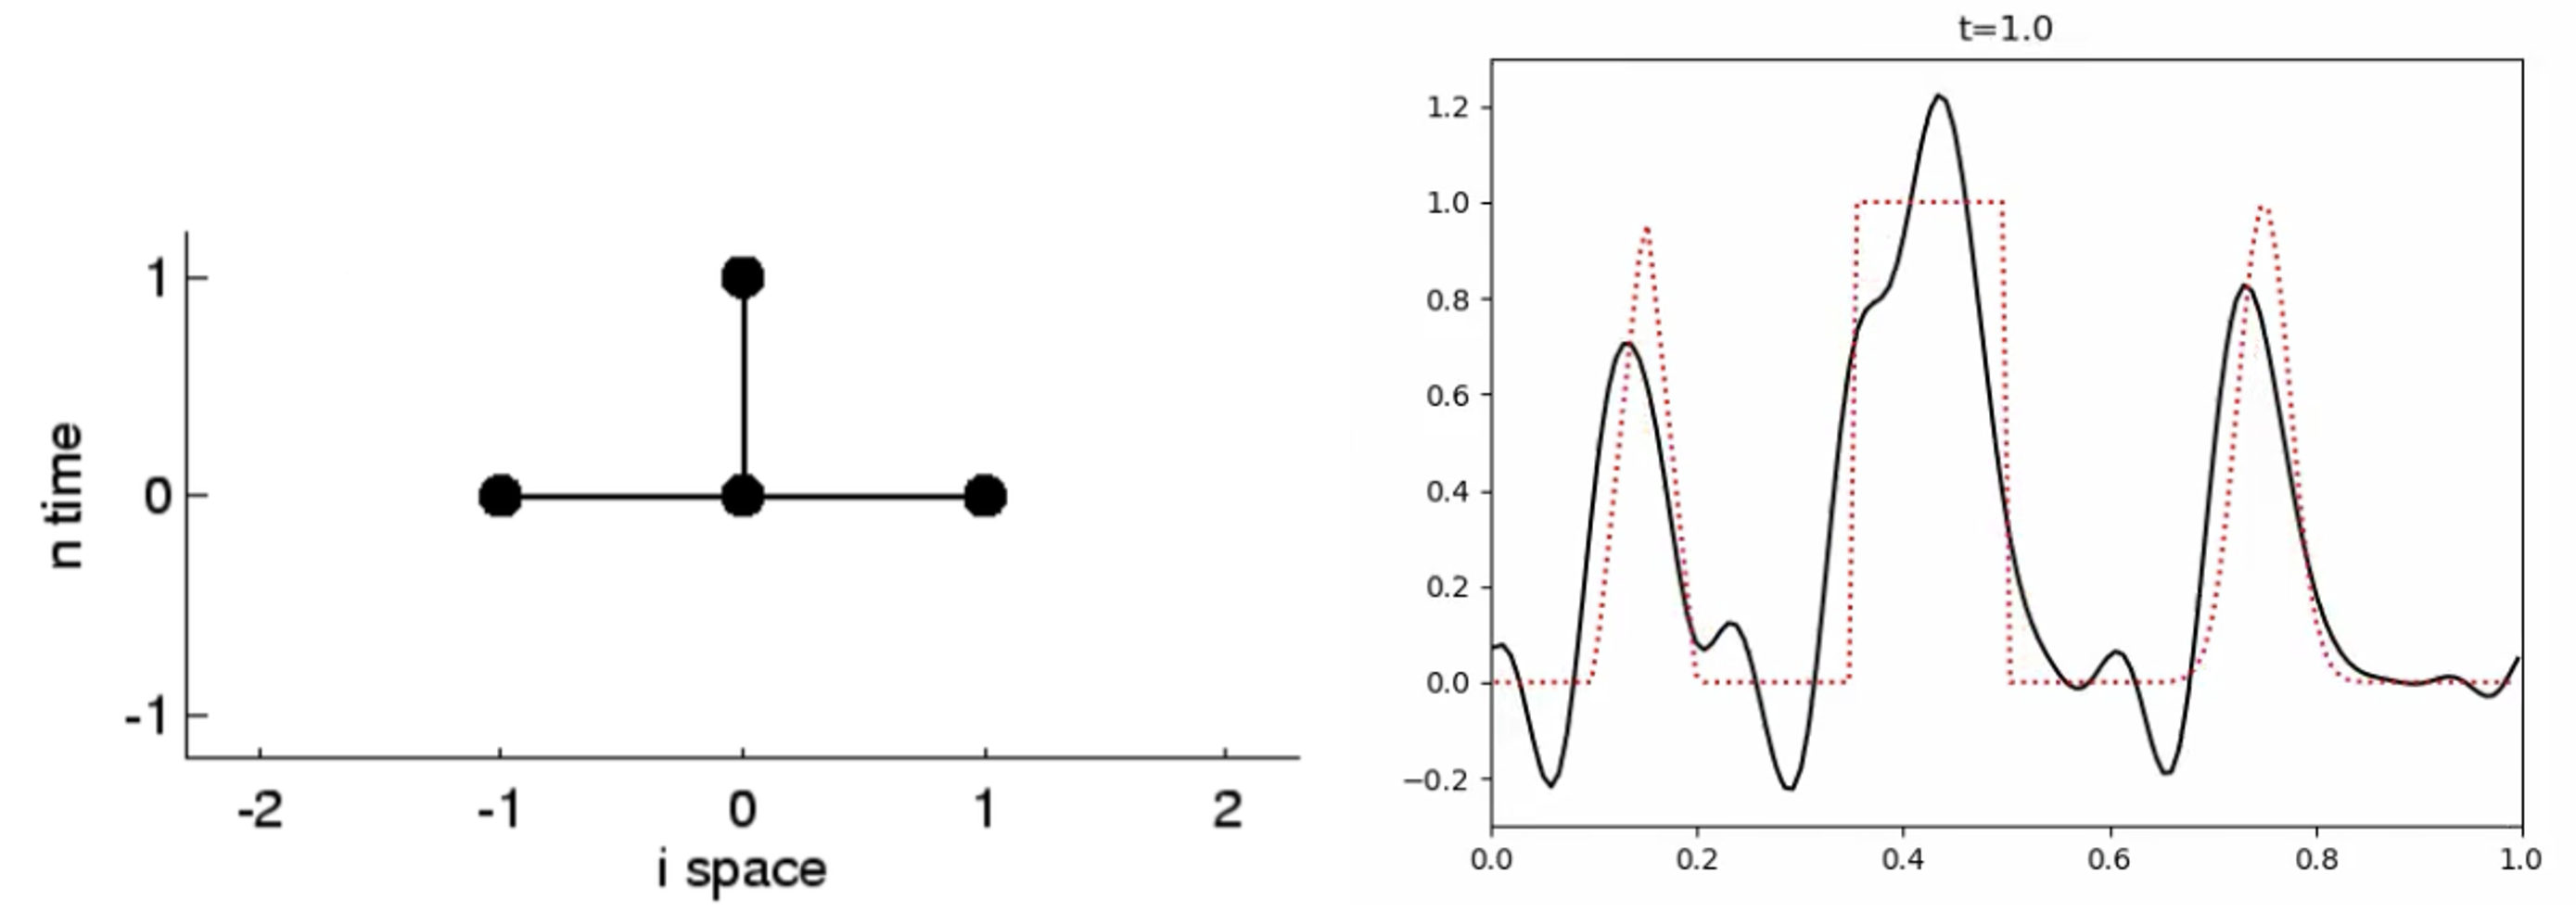
\includegraphics{./figs/laxwendroff.png}}
  \end{center}
  \caption[]{Lax-Wendroff}
  \label{fig:lax-wendroff}
\end{figure}

The result is smooth \figp{fig:lax-wendroff} with considerable overshoot (that, however, does not grow in time). This scheme might be useful for more regular initial conditions.

\subsection{Beam-Warming}

The Beam-Warming scheme \figp{fig:beam-warming} uses the backward slope

\begin{equation}
\delta q_i = \delta q_{\rm backward} = q_{i} - q_{i-1}
\end{equation}

\begin{figure}
  \begin{center}
    \resizebox{\textwidth}{!}{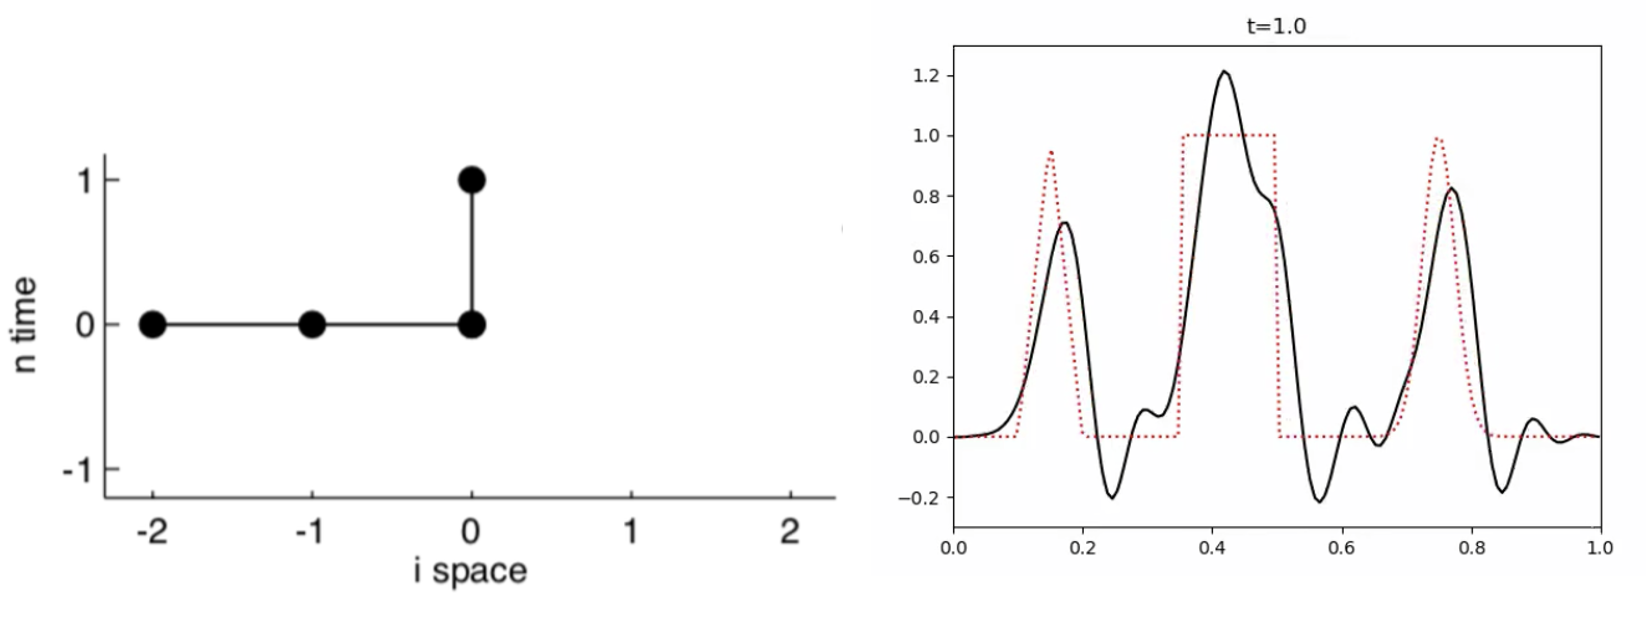
\includegraphics{./figs/beam-warming.png}}
  \end{center}
  \caption[]{Beam-Warming}
  \label{fig:beam-warming}
\end{figure}

\subsection{Fromm}

The Fromm scheme is the average of forward and backward

\begin{equation}
\delta q_i = \frac{1}{2}\left(\delta q_{\rm forward}+\delta q_{\rm backward}\right)
\end{equation}

\begin{figure}
  \begin{center}
    \resizebox{\textwidth}{!}{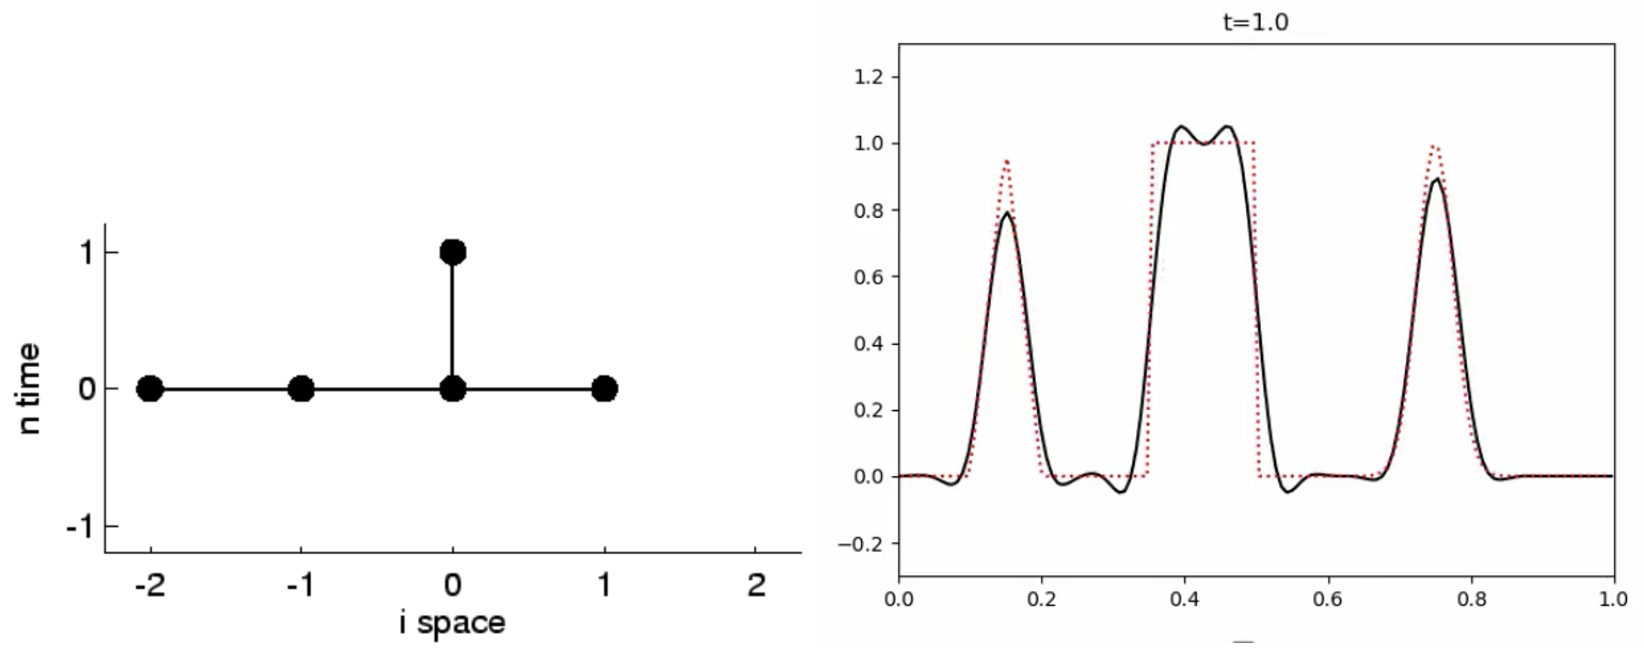
\includegraphics{./figs/fromm.png}}
  \end{center}
  \caption[]{Fromm}
  \label{fig:fromm}
\end{figure}

The result is smooth with some amount of overshoot \figp{fig:fromm}. The initial shape
of the spikes is recognizable. So far the best scheme, if the
overshoot can be accepted.

\subsection{Nonlinear Slopes}

The nonlinear schemes are also called {\bf slope limiters}. They are
non-linear tools to prevent overshoots. With the current piecewise linear geometric picture of the higher
order methods we can gain a geometrical understanding of why such an overshoot occurs. 

In this picture the overshoot happens because the piecewise linear elements can have overshoots. A succesful method to prevent such overshoots is the use of slope limiters. These are
non-linear conditions that modify the slope if, and only if, this is necessary to prevent overshoots. This means that, if this is applied to for instance the Lax-Wendroff method, the slope
limiter keeps the higher (2nd) order nature of the Lax-Wendroff method in regions of smooth variation
of $q$ while it will intervene whenever an overshoot threatens to take place.

In these
schemes, nonlinear corrections are inserted with the purpose of
hindering the oscillations from going unstable. The way these schemes
achieve this result is by limiting the slope to well-behaved
values. We will try three slope limiters: MinMod, Van Leer, and
Superbee.

\subsubsection{MinMod}

In the MinMod slope limiter, the slope is determined by 

\begin{eqnarray}
\delta q_i &=& \mathrm{min}[\mathrm{max} (\delta q_f,0),\mathrm{max}(\delta q_b,0)] \\
&+& \mathrm{max}[\mathrm{min} (\delta q_f,0),\mathrm{min}(\delta q_b,0)]
\end{eqnarray}

\begin{figure}
  \begin{center}
    \resizebox{\textwidth}{!}{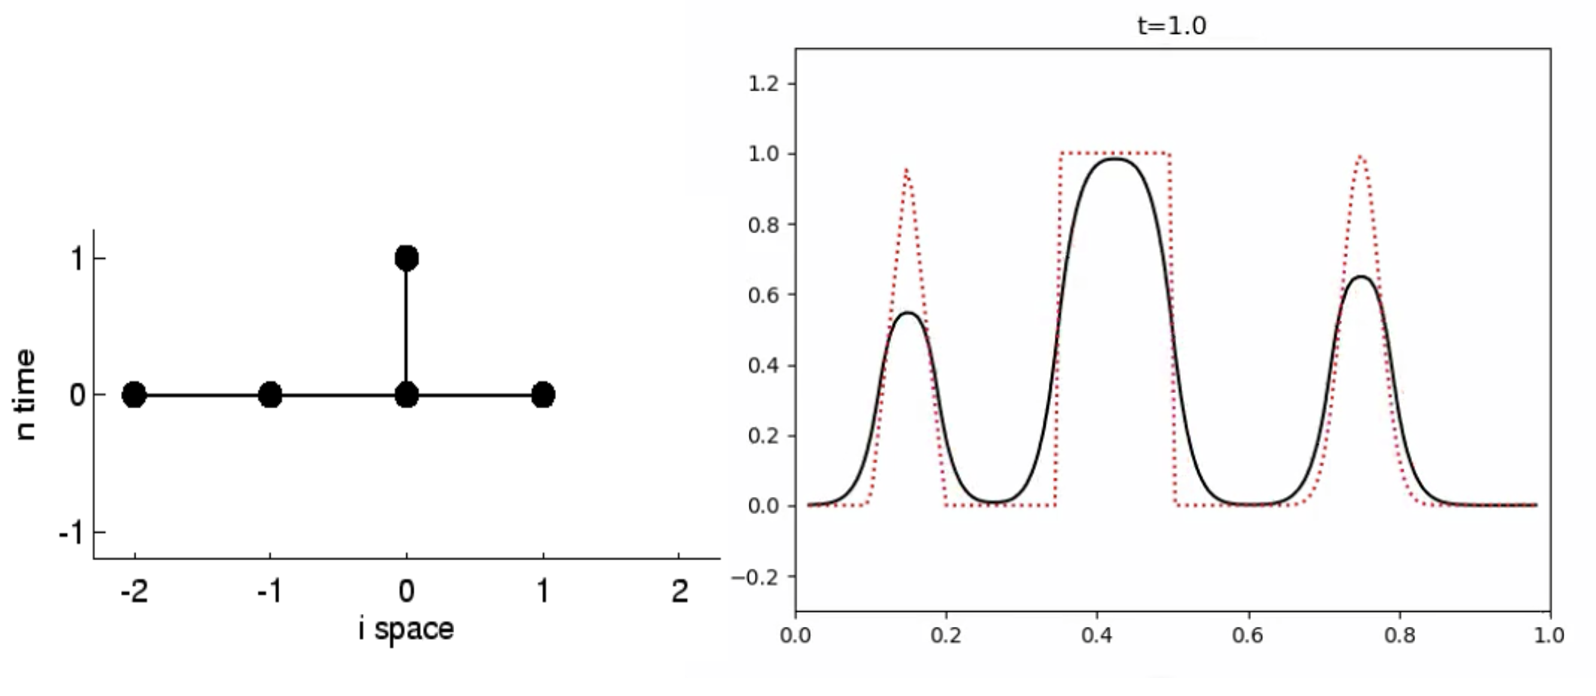
\includegraphics{./figs/minmod.png}}
  \end{center}
  \caption[]{Minmod}
  \label{fig:minmod}
\end{figure}

This method chooses the smallest of the two slopes, provided they both have the same sign, and
chooses 0 otherwise.

\subsubsection{Van Leer}

\begin{equation}
\delta q_i = \left\{
\begin{array}{ccc}
\frac{2}{\delta q_f^{-1} + \delta q_b^{-1}} & \quad & \mathrm{if} \quad \delta q_f \delta q_b > 0  \\
0 &\quad & \mathrm{if} \quad  \delta q_f \delta q_b \leq 0
\end{array}\right.
\end{equation}

\begin{figure}
  \begin{center}
    \resizebox{\textwidth}{!}{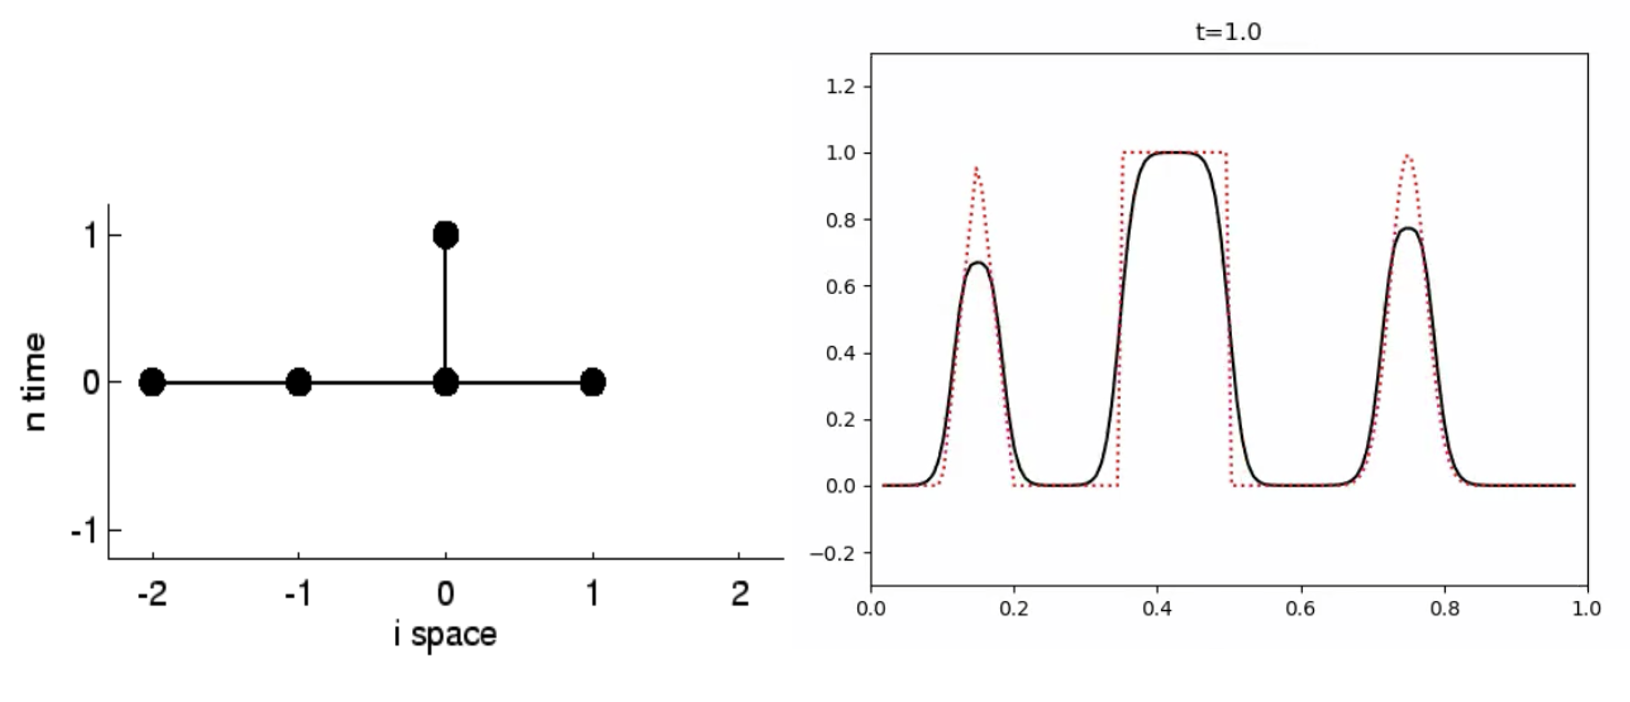
\includegraphics{./figs/vanleer.png}}
  \end{center}
  \caption[]{Van Leer}
  \label{fig:vanleer}
\end{figure}

\subsubsection{Superbee}

\begin{equation}
\delta q_i = \left[\mbox{sign}(\delta q_f) + \mbox{sign}(\delta q_b)\right] \times 
\mathrm{min} \left\{ \mbox{abs}(\delta q_f), \mbox{abs}(\delta q_b), \frac{1}{2} \mbox{max} \left[\mbox{abs}(\delta q_f),\mathrm{abs}\left(\delta q_b\right) \right]\right\}
\end{equation}


\begin{figure}
  \begin{center}
    \resizebox{\textwidth}{!}{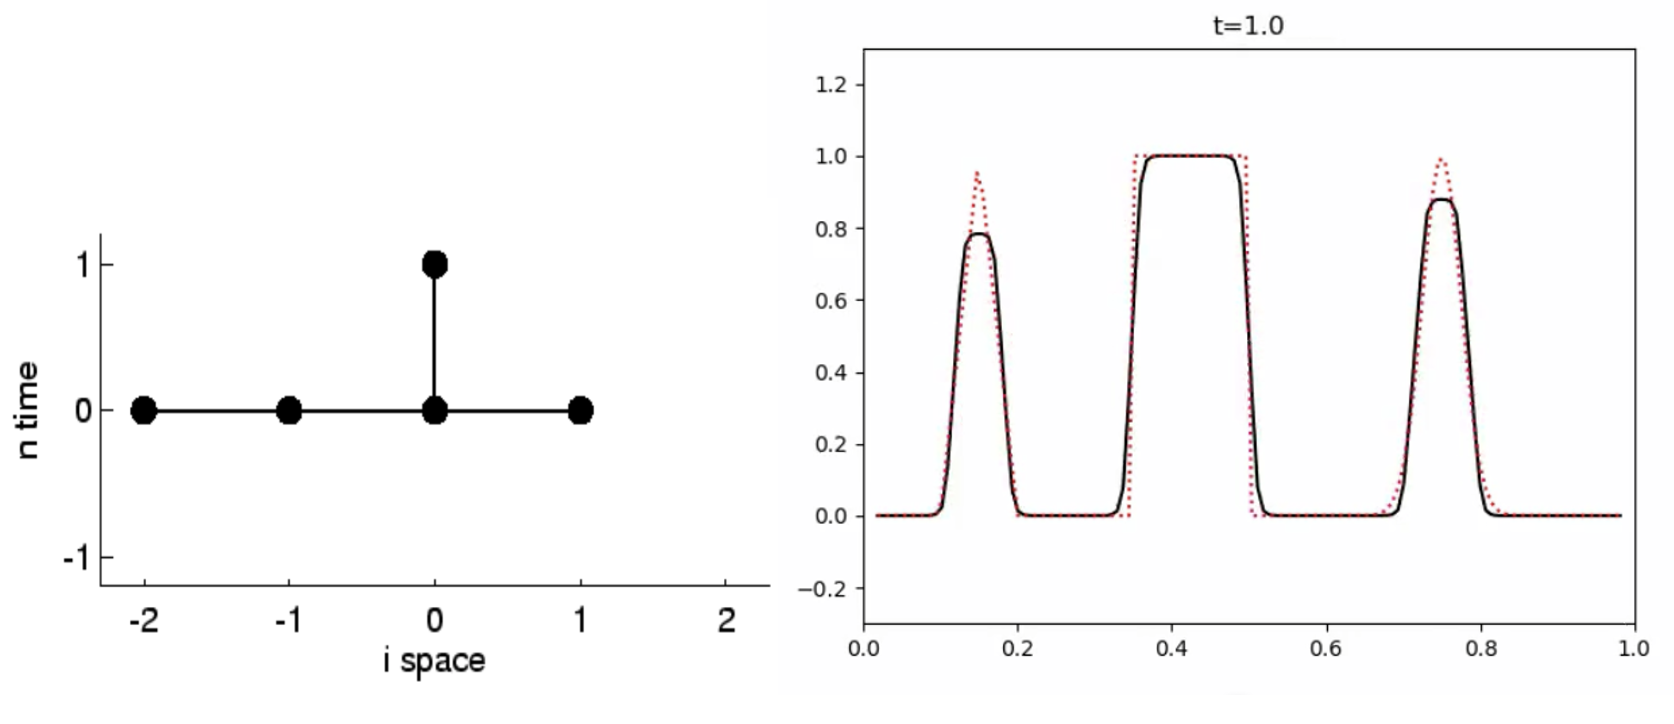
\includegraphics{./figs/superbee.png}}
  \end{center}
  \caption[]{Superbee}
  \label{fig:superbee}
\end{figure}

\subsection{Exercises}

\subsubsection{The stable schemes}

\begin{itemize}

\item Use a Gaussian ( $e^{-\left(x/0.1\right)^2}$) and a rectangle ( $1 \mbox{ for abs}(x) < 0.2 \mbox{ and } 0 \mbox{ elsewhere}$) as initial conditions. 

\item  Use a reasonable Courant number (e.g. $C=0.4$) and keep it fixed. Simulate a complete 
revolution ( $v\Delta T    = 1$) to facilitate the comparison with the exact final result (= initial condition).

\item  Compare the results for different resolutions (e.g. 25, 50, 100, 200 grid points).

\item  Measure the error with the following norms

\begin{itemize}
  
\item The 1-norm

\begin{equation}
N_1 = \frac{1}{N} \sum_i^N \mbox{abs}\left(q_i^{(t)} - q_i^{(0)}\right)
\end{equation}

\item The Euclidian 2-norm 

\begin{equation}
N_2 = \frac{1}{N} \left[\sum_i^N \mbox{abs}\left(q_i^{(t)} - q_i^{(0)}\right)^2\right]^{1/2}
\end{equation}

\item and the maximum-norm 


\begin{equation}
N_\mathrm{max} = \mbox{max abs} \left(q_i^{(t)} - q_i^{(0)}\right)
\end{equation}

\end{itemize}

\end{itemize}
